
%\documentclass[11pts,a4paper,amsmath,amssymb,floatfix]{article}%{report}%{book}
\documentclass[12pts,a4paper,amsmath,amssymb,floatfix]{article}%{report}%{book}
\usepackage{graphicx}
\usepackage{wrapfig,pdfpages}% Include figure files
%\usepackage{dcolumn,enumerate}% Align table columns on decimal point
\usepackage{enumerate,enumitem}% Align table columns on decimal point
\usepackage{bm,dpfloat}% bold math
%\usepackage[pdftex,bookmarks,colorlinks=true,urlcolor=rltblue,citecolor=blue]{hyperref}
\usepackage{amsfonts,amsmath,amssymb,stmaryrd,indentfirst}
\usepackage{times,psfrag}
\usepackage{natbib}
\usepackage{color}
\usepackage{units}
\usepackage{rotating}
\usepackage{multirow}


\usepackage{pifont}
\usepackage{subfigure}
\usepackage{subeqnarray}
\usepackage{ifthen}

\usepackage{supertabular}
\usepackage{moreverb}
\usepackage{listings}
\usepackage{palatino}
%\usepackage{doi}
\usepackage{longtable}
\usepackage{float}
\usepackage{perpage}
\MakeSorted{figure}
%\usepackage{pdflscape}
\usepackage{soul} %% use \hl to higlight text

%\usepackage{booktabs}
%\newcommand{\ra}[1]{\renewcommand{\arraystretch}{#1}}


\definecolor{rltblue}{rgb}{0,0,0.75}


%\usepackage{natbib}
\usepackage{fancyhdr} %%%%
\pagestyle{fancy}%%%%
% with this we ensure that the chapter and section
% headings are in lowercase
%%%%\renewcommand{\chaptermark}[1]{\markboth{#1}{}}
\renewcommand{\sectionmark}[1]{\markright{\thesection\ #1}}
\fancyhf{} %delete the current section for header and footer
\fancyhead[LE,RO]{\bfseries\thepage}
\fancyhead[LO]{\bfseries\rightmark}
\fancyhead[RE]{\bfseries\leftmark}
\renewcommand{\headrulewidth}{0.5pt}
% make space for the rule
\fancypagestyle{plain}{%
\fancyhead{} %get rid of the headers on plain pages
\renewcommand{\headrulewidth}{0pt} % and the line
}

\def\newblock{\hskip .11em plus .33em minus .07em}
\usepackage{color}

%\usepackage{makeidx}
%\makeindex

\setlength\textwidth      {16.cm}
\setlength\textheight     {22.6cm}
\setlength\oddsidemargin  {-0.3cm}
\setlength\evensidemargin {0.3cm}

\setlength\headheight{14.49998pt}
\setlength\topmargin{0.0cm}
\setlength\headsep{1.cm}
\setlength\footskip{1.cm}
\setlength\parskip{0pt}
\setlength\parindent{0pt}


%%%
%%% Headers and Footers
\lhead[] {\text{\small{EG501V -- Computational Fluid Dynamics}}}
\rhead[\text{\small{Assignment}}]{Assignment}
%\rfoot[] {{\text{\small{EOS + Mass Conservation using Matlab }}}}
%\chead[] {\text{\small{Session 2012/13}}}
\lfoot[]{CFD: Laminar and Turbulent Jets}
\rfoot[\thepage]{\thepage}
\renewcommand{\headrulewidth}{0.8pt}


%%%
%%% space between lines
%%%
\renewcommand{\baselinestretch}{1.5}

\newenvironment{VarDescription}[1]%
  {\begin{list}{}{\renewcommand{\makelabel}[1]{\textbf{##1:}\hfil}%
    \settowidth{\labelwidth}{\textbf{#1:}}%
    \setlength{\leftmargin}{\labelwidth}\addtolength{\leftmargin}{\labelsep}}}%
  {\end{list}}

%%%%%%%%%%%%%%%%%%%%%%%%%%%%%%%%%%%%%%%%%%%
%%%%%%                              %%%%%%%
%%%%%%      NOTATION SECTION        %%%%%%%
%%%%%%                              %%%%%%%
%%%%%%%%%%%%%%%%%%%%%%%%%%%%%%%%%%%%%%%%%%%

% Text abbreviations.
\newcommand{\ie}{{\em{i.e., }}}
\newcommand{\eg}{{\em{e.g., }}}
\newcommand{\cf}{{\em{cf., }}}
\newcommand{\wrt}{with respect to}
\newcommand{\lhs}{left hand side}
\newcommand{\rhs}{right hand side}
% Commands definining mathematical notation.

% This is for quantities which are physically vectors.
\renewcommand{\vec}[1]{{\mbox{\boldmath$#1$}}}
% Physical rank 2 tensors
\newcommand{\tensor}[1]{\overline{\overline{#1}}}
% This is for vectors formed of the value of a quantity at each node.
\newcommand{\dvec}[1]{\underline{#1}}
% This is for matrices in the discrete system.
\newcommand{\mat}[1]{\mathrm{#1}}


\DeclareMathOperator{\sgn}{sgn}
\newtheorem{thm}{Theorem}[section]
\newtheorem{lemma}[thm]{Lemma}

%\newcommand\qed{\hfill\mbox{$\Box$}}
\newcommand{\re}{{\mathrm{I}\hspace{-0.2em}\mathrm{R}}}
\newcommand{\inner}[2]{\langle#1,#2\rangle}
\renewcommand\leq{\leqslant}
\renewcommand\geq{\geqslant}
\renewcommand\le{\leqslant}
\renewcommand\ge{\geqslant}
\renewcommand\epsilon{\varepsilon}
\newcommand\eps{\varepsilon}
\renewcommand\phi{\varphi}
\newcommand{\bmF}{\vec{F}}
\newcommand{\bmphi}{\vec{\phi}}
\newcommand{\bmn}{\vec{n}}
\newcommand{\bmns}{{\textrm{\scriptsize{\boldmath $n$}}}}
\newcommand{\bmi}{\vec{i}}
\newcommand{\bmj}{\vec{j}}
\newcommand{\bmk}{\vec{k}}
\newcommand{\bmx}{\vec{x}}
\newcommand{\bmu}{\vec{u}}
\newcommand{\bmv}{\vec{v}}
\newcommand{\bmr}{\vec{r}}
\newcommand{\bma}{\vec{a}}
\newcommand{\bmg}{\vec{g}}
\newcommand{\bmU}{\vec{U}}
\newcommand{\bmI}{\vec{I}}
\newcommand{\bmq}{\vec{q}}
\newcommand{\bmT}{\vec{T}}
\newcommand{\bmM}{\vec{M}}
\newcommand{\bmtau}{\vec{\tau}}
\newcommand{\bmOmega}{\vec{\Omega}}
\newcommand{\pp}{\partial}
\newcommand{\kaptens}{\tensor{\kappa}}
\newcommand{\tautens}{\tensor{\tau}}
\newcommand{\sigtens}{\tensor{\sigma}}
\newcommand{\etens}{\tensor{\dot\epsilon}}
\newcommand{\ktens}{\tensor{k}}
\newcommand{\half}{{\textstyle \frac{1}{2}}}
\newcommand{\tote}{E}
\newcommand{\inte}{e}
\newcommand{\strt}{\dot\epsilon}
\newcommand{\modu}{|\bmu|}
% Derivatives
\renewcommand{\d}{\mathrm{d}}
\newcommand{\D}{\mathrm{D}}
\newcommand{\ddx}[2][x]{\frac{\d#2}{\d#1}}
\newcommand{\ddxx}[2][x]{\frac{\d^2#2}{\d#1^2}}
\newcommand{\ddt}[2][t]{\frac{\d#2}{\d#1}}
\newcommand{\ddtt}[2][t]{\frac{\d^2#2}{\d#1^2}}
\newcommand{\ppx}[2][x]{\frac{\partial#2}{\partial#1}}
\newcommand{\ppxx}[2][x]{\frac{\partial^2#2}{\partial#1^2}}
\newcommand{\ppt}[2][t]{\frac{\partial#2}{\partial#1}}
\newcommand{\pptt}[2][t]{\frac{\partial^2#2}{\partial#1^2}}
\newcommand{\DDx}[2][x]{\frac{\D#2}{\D#1}}
\newcommand{\DDxx}[2][x]{\frac{\D^2#2}{\D#1^2}}
\newcommand{\DDt}[2][t]{\frac{\D#2}{\D#1}}
\newcommand{\DDtt}[2][t]{\frac{\D^2#2}{\D#1^2}}
% Norms
\newcommand{\Ltwo}{\ensuremath{L_2} }
% Basis functions
\newcommand{\Qone}{\ensuremath{Q_1} }
\newcommand{\Qtwo}{\ensuremath{Q_2} }
\newcommand{\Qthree}{\ensuremath{Q_3} }
\newcommand{\QN}{\ensuremath{Q_N} }
\newcommand{\Pzero}{\ensuremath{P_0} }
\newcommand{\Pone}{\ensuremath{P_1} }
\newcommand{\Ptwo}{\ensuremath{P_2} }
\newcommand{\Pthree}{\ensuremath{P_3} }
\newcommand{\PN}{\ensuremath{P_N} }
\newcommand{\Poo}{\ensuremath{P_1P_1} }
\newcommand{\PoDGPt}{\ensuremath{P_{-1}P_2} }

\newcommand{\metric}{\tensor{M}}
\newcommand{\configureflag}[1]{\texttt{#1}}

% Units
\newcommand{\m}[1][]{\unit[#1]{m}}
\newcommand{\km}[1][]{\unit[#1]{km}}
\newcommand{\s}[1][]{\unit[#1]{s}}
\newcommand{\invs}[1][]{\unit[#1]{s}\ensuremath{^{-1}}}
\newcommand{\ms}[1][]{\unit[#1]{m\ensuremath{\,}s\ensuremath{^{-1}}}}
\newcommand{\mss}[1][]{\unit[#1]{m\ensuremath{\,}s\ensuremath{^{-2}}}}
\newcommand{\K}[1][]{\unit[#1]{K}}
\newcommand{\PSU}[1][]{\unit[#1]{PSU}}
\newcommand{\Pa}[1][]{\unit[#1]{Pa}}
\newcommand{\kg}[1][]{\unit[#1]{kg}}
\newcommand{\rads}[1][]{\unit[#1]{rad\ensuremath{\,}s\ensuremath{^{-1}}}}
\newcommand{\kgmm}[1][]{\unit[#1]{kg\ensuremath{\,}m\ensuremath{^{-2}}}}
\newcommand{\kgmmm}[1][]{\unit[#1]{kg\ensuremath{\,}m\ensuremath{^{-3}}}}
\newcommand{\Nmm}[1][]{\unit[#1]{N\ensuremath{\,}m\ensuremath{^{-2}}}}

% Dimensionless numbers
\newcommand{\dimensionless}[1]{\mathrm{#1}}
\renewcommand{\Re}{\dimensionless{Re}}
\newcommand{\Ro}{\dimensionless{Ro}}
\newcommand{\Fr}{\dimensionless{Fr}}
\newcommand{\Bu}{\dimensionless{Bu}}
\newcommand{\Ri}{\dimensionless{Ri}}
\renewcommand{\Pr}{\dimensionless{Pr}}
\newcommand{\Pe}{\dimensionless{Pe}}
\newcommand{\Ek}{\dimensionless{Ek}}
\newcommand{\Gr}{\dimensionless{Gr}}
\newcommand{\Ra}{\dimensionless{Ra}}
\newcommand{\Sh}{\dimensionless{Sh}}
\newcommand{\Sc}{\dimensionless{Sc}}



% Journals
\newcommand{\IJHMT}{{\it International Journal of Heat and Mass Transfer}}
\newcommand{\NED}{{\it Nuclear Engineering and Design}}
\newcommand{\ICHMT}{{\it International Communications in Heat and Mass Transfer}}
\newcommand{\NET}{{\it Nuclear Engineering and Technology}}
\newcommand{\HT}{{\it Heat Transfer}}
\newcommand{\IJHT}{{\it International Journal for Heat Transfer}}

\newcommand{\frc}{\displaystyle\frac}
\newcommand{\red}{\textcolor{red}}
\newcommand{\blue}{\textcolor{blue}}
\newcommand{\green}{\textcolor{green}}
\newcommand{\purple}{\textcolor{purple}}

\newlist{ExList}{enumerate}{1}
\setlist[ExList,1]{label={\bf Example 1.} {\bf \arabic*}}

\newlist{ProbList}{enumerate}{1}
\setlist[ProbList,1]{label={\bf Problem 1.} {\bf \arabic*}}

%%%%%%%%%%%%%%%%%%%%%%%%%%%%%%%%%%%%%%%%%%%
%%%%%%                              %%%%%%%
%%%%%% END OF THE NOTATION SECTION  %%%%%%%
%%%%%%                              %%%%%%%
%%%%%%%%%%%%%%%%%%%%%%%%%%%%%%%%%%%%%%%%%%%


% Cause numbering of subsubsections.
%\setcounter{secnumdepth}{8}
%\setcounter{tocdepth}{8}

\setcounter{secnumdepth}{4}%
\setcounter{tocdepth}{4}%


\begin{document}

\begin{enumerate}[label=\bfseries Problem \arabic*:]
%%%
%%% PROBLEM 1
%%%
   \item\label{Problem1} {\bf Simulation and Analysis of Idealised Laminar and Turbulent Free Jets}

In this problem, laminar and turbulent free jets will be simulated in a prescribed 2-D axisymmetric geometry. The term `free' means that the jet flow enters a domain unconfined by any boundaries. The simulated domain, Fig.~\ref{EG501V_Assignment:Sketch1}, has a length of 1.0 m and low and high width of 0.205 and 0.305 m, respectively. Line AD is the centerline of the full domain.

Air is injected through a narrow inlet region on the left-hand side border (AB) with a prescribed inlet velocity. Boundary conditions can be summarised as (a) no flux is allowed across border AD %and BC \hl{(there is flux across BC I think? - it is a pressure inlet}) 
and (b) Dirichlet radial fluid velocity at border (AB),
         \[ u_{x}( x=0, y, t) = \begin{cases}
             1\,m/s & \text{ if } \;\;\;0\leq y\leq 0.005 \text{ m}; \\
             0\,m/s & \text{ elsewhere.}
         \end{cases}\]
        % \hl{mention what boundary CD is?}
We can consider that, initially, the domain contains air at rest, i.e., $\underline{u}\left(\underline{x},t=0\right)=0$. Two case-scenarios will be analysed here, laminar and turbulent jets. Initial mesh and simulation setup can be downloaded from {\it MyAberdeen}.


\begin{figure}[h]
\begin{center}
%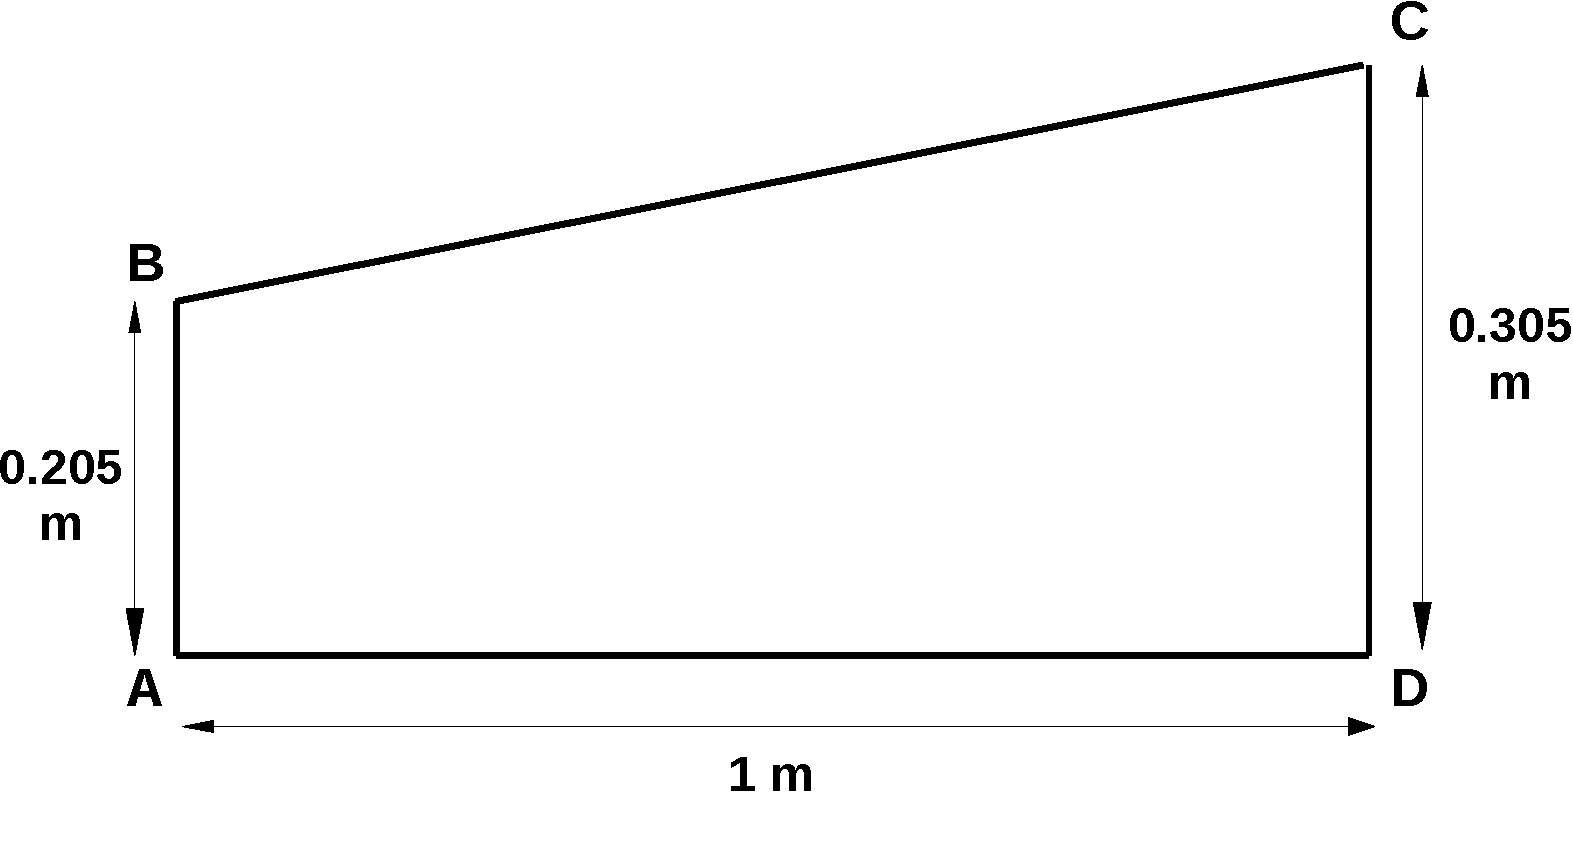
\includegraphics[width=15.cm,height=8.cm,clip]{./Pics/Sketch_Prob1b}
%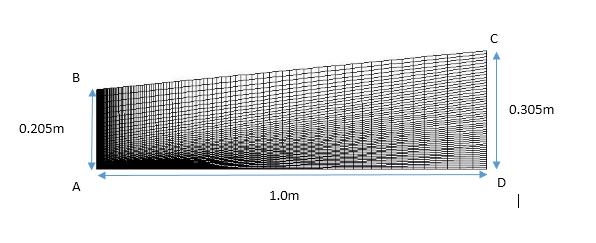
\includegraphics[width=15.cm,height=8.cm,clip]{./Pics/mesh.png}
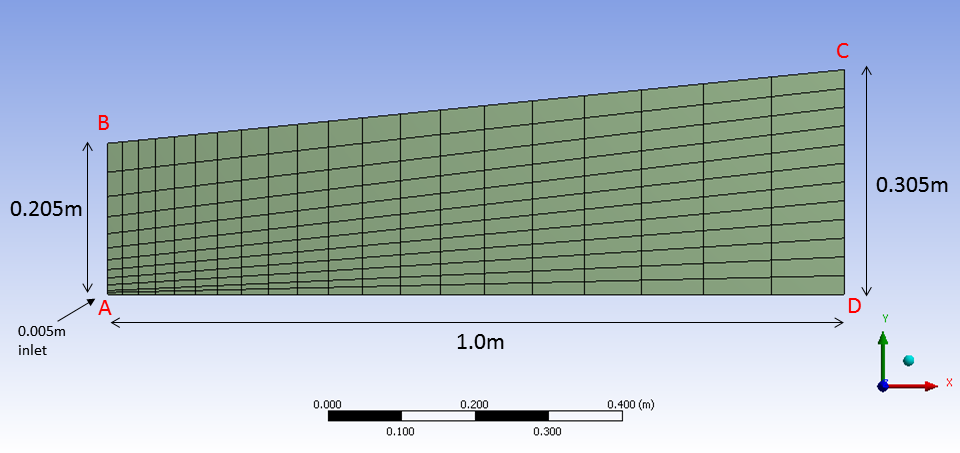
\includegraphics[width=14.cm,height=8.cm,clip]{./Pics/free_jet_mesh.png}
\caption{Initial sketch of the free jet simulation problem. }
\label{EG501V_Assignment:Sketch1}
\end{center}
\end{figure}

\begin{enumerate}[label=\bfseries Task 1.\arabic*]

%%% Task 1
\item\label{Practical1:Task1} {\bf Laminar Free Jet}
  \begin{enumerate}
     \item Check if the flow is laminar;
     \item\label{Task1:MeshIndependenceCriteria} Check for mesh-independence:
        \begin{itemize}
            \item Perform the simulation with the current setup and plot {\it velocity magnitude} $\times$ {\it x-position} $\left(\mathbf{u}\times\mathbf{X}\right)$ along the centreline;
            \item Smoothly increase the mesh resolution (i.e., refine the mesh), re-run the simulation and plot the resulting $\mathbf{u}\times\mathbf{X}$;
            \item Repeat this procedure until the computed solution is mesh-independent;
            \item The solution is considered to be mesh-independent when there is no change in calculated fields as the grid is refined, i.e., no changes in the $\mathbf{u}\times\mathbf{X}$ plot;
        \end{itemize}
     \item From the simulation performed with the final mesh, plot $\left(\frc{\mathbf{u}}{\mathbf{u}_{\text{max}}}\times \frc{\mathbf{X}}{\mathbf{D}}\right)$, where $\mathbf{u}_{\text{max}}$ is the maximum velocity and $\mathbf{D}=$ 0.01 m is the nozzle inlet diameter (= characteristic length-scale).
     \item\label{Task1:StreamFunction} Also, obtain the contour plot of the stream function;
     \item Repeat the simulation using 1$^{\text{st}}$-order accurate scheme for the momentum equation and compare the plots.
  \end{enumerate}

%%% Task 2
\item\label{Practical1:Task2} {\bf Turbulent Free Jet}
  \begin{enumerate}
     \item Using the same initial simulation set-up used in~\ref{Practical1:Task1} (including fluid density, inlet velocity and diameter), modify the simulation conditions to ensure a Reynolds number of 10$^{5}$;
     \item Use the standard $k-\epsilon$ turbulence model. The $k-\epsilon$ terms must be specified on all boundaries;
     \item In {\it Solution Setup} $\rightarrow$ {\it Boundary Conditions}, edit both {\it Farfield} and {\it Inlet boundaries}. Select {\it `Intensity and Hydraulic Diameter'} as the turbulence specification method;
     \item At the {\it Inlet 1} windows, modify the {\it Specification Method} for {\it Turbulence} to \blue{\it Intensity and Hydraulic Diameter}. The intensity should be $I=5\%$, and the hydraulic diameter should be $d_{H}=0.01 m$;
     \item At the {\it Inlet 2} and {\it Farfield} boundaries windows, modify the {\it Specification Method} for {\it Turbulence} to \blue{\it K and Epsilon}. Both should be zero;
     \item In the {\it `Monitors'}, edit the residual monitors and ensure that the residual criteria for both $k$ and $\epsilon$ are 10$^{-6}$;
     \item Repeat steps \red{(ii)}-\red{(iv)} from~\ref{Practical1:Task1};
     \item Plot the turbulent kinetic energy along the centreline, i.e., $k\times\mathbf{X}$;
     \item Plot $\left(\frc{\mathbf{u}}{\mathbf{u}_{\text{max}}}\times \frc{\mathbf{X}}{\mathbf{D}}\right)$ for $Re=\left[ 10^{2}\; 10^{3}\; 10^{4}\; 10^{5}\; 10^{6}\right]$. 
  \end{enumerate}
\end{enumerate}

\clearpage

%%%
%%% PROBLEM 2
%%%
   \item\label{Problem2} {\bf Simulation of Idealised 2-D Waste Flow Discharge}

A team of engineers and consultants are designing a new industrial unit near the coast (Fig.~\ref{EG501V_Assignment:Sketch2}). Cold sea water is used as cooling fluid for main the process and all for heat exchangers and condensers of the unit, and then returned back to the sea through a pipeline of 0.5 m diameter at 700 m$^{3}$/h (properties of returned water and sea water are assumed the same, $\rho=$ 1000 kg/m$^{3}$, $\mu=$ 0.001 kg/(m.s)). The seabed consists of uniform sand with mean diameter $D_{50}$ of 0.001 m.

\begin{figure}[h]
\vbox{\hbox{\hspace{2cm}
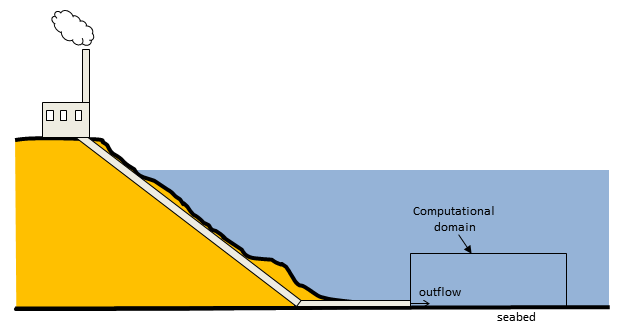
\includegraphics[width=13.cm,height=8.cm,clip]{./Pics/problem_sketch.png}}
\vspace{-0.cm}
\hbox{\hspace{3cm}
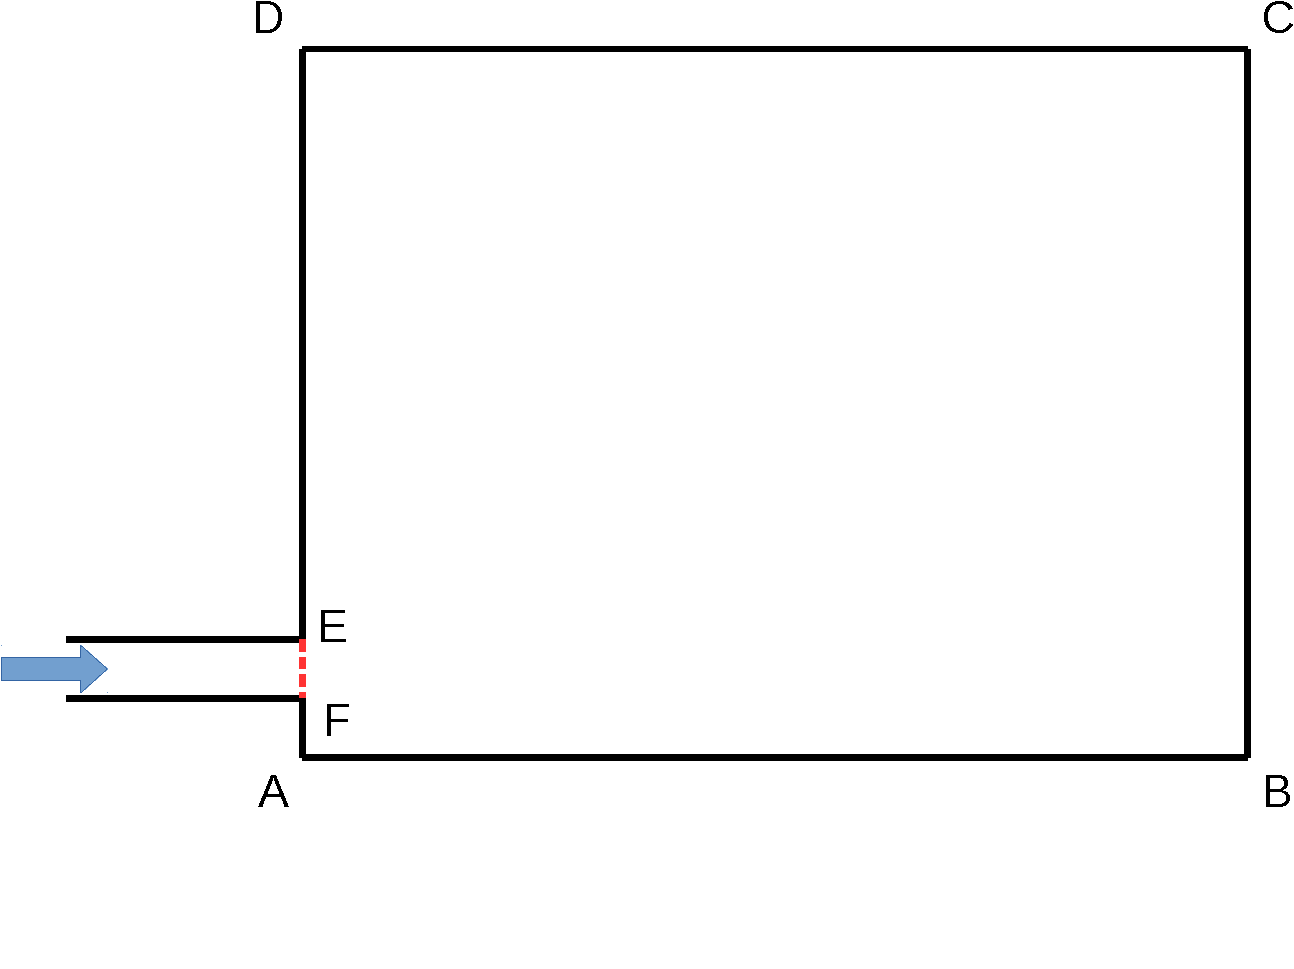
\includegraphics[width=10.cm,height=6.cm,clip]{./Pics/Sketch_Prob2b}}}\vspace{-1.5cm}
\caption{Physical domain of the waste flow discharge (top) and initial sketch of simulation problem. Dimensions are: $\overline{AB}=$ 50.0 m, $\overline{BC}=$ 8.0 m, $\overline{DE}=$ 7.5 m, $\overline{EF}=$ 0.5 m and $\overline{AF}=$ 0.0 m.} \label{EG501V_Assignment:Sketch2}
\end{figure}

%\begin{figure}[h]
%\begin{center}
%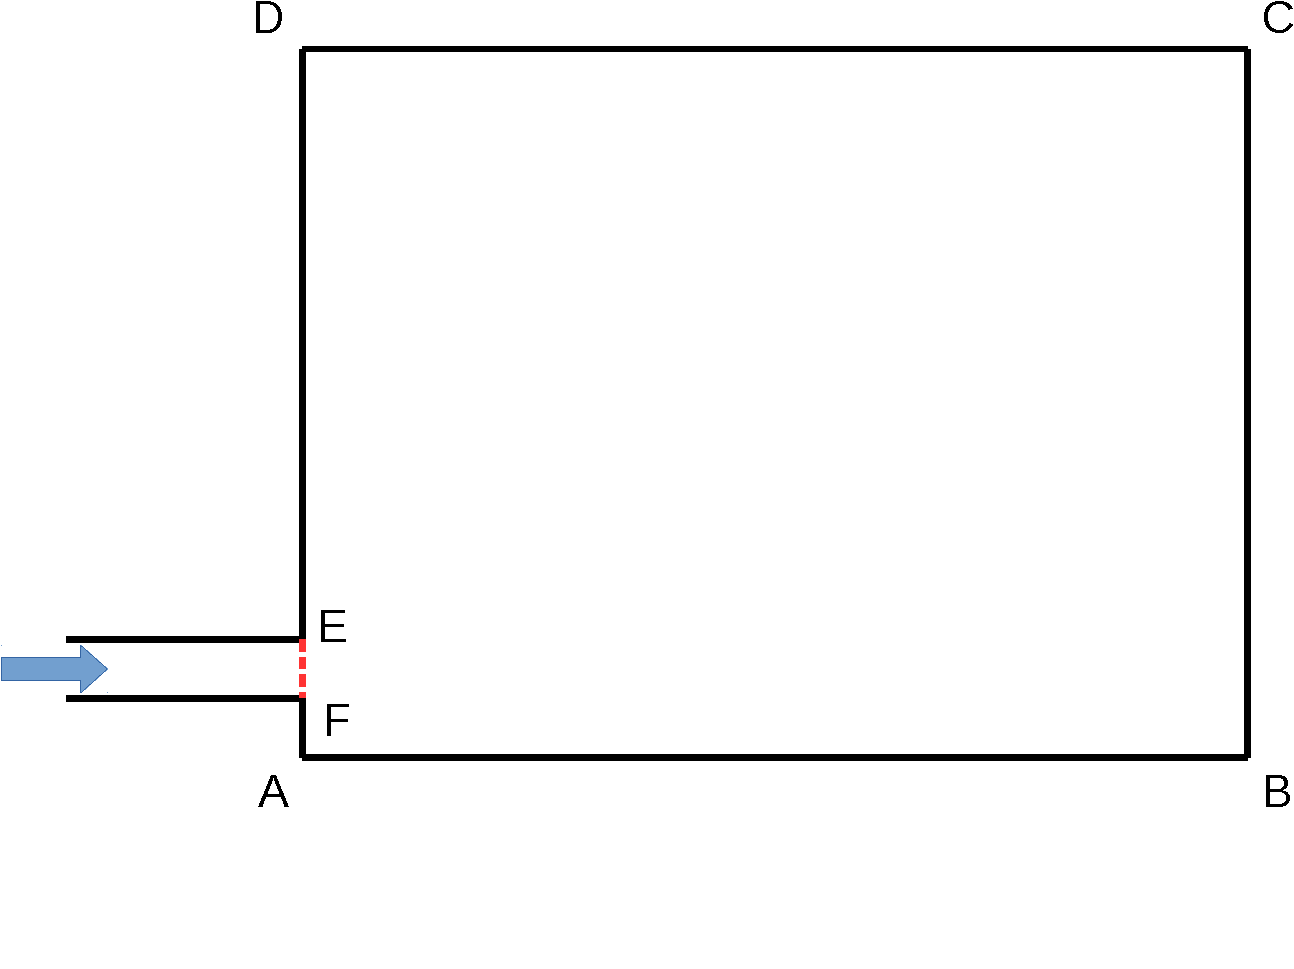
\includegraphics[width=13.cm,height=8.cm,clip]{./Pics/Sketch_Prob2b}\vspace{-1.5cm}
%\caption{Initial sketch of the waste flow discharge simulation problem. The dimensions are: $\overline{AB}=$ 50.0 m, $\overline{BC}=$ 8.0 m, $\overline{DE}=$ 7.5 m, $\overline{EF}=$ 0.5 m and $\overline{AF}=$ 0.0 m.} \label{EG501V_Assignment:Sketch2}
%\end{center}
%\end{figure}

To study the effect of the discharged flow on the surrounding environment the team decided to simplify the problem to a rectangular domain (ABCD in Fig.~\ref{EG501V_Assignment:Sketch2}) assuming that the waste water is introduced through an inlet ($\overline{EF}$ in Fig.~\ref{EG501V_Assignment:Sketch2}) as fully developed turbulent flow with $Re=$ 5$\times$10$^{5}$. Boundary conditions may be summarised as,
\begin{itemize}
  \item Non-slip (wall) condition in $\overline{\text{AB}}$;
  \item Outflow (pressure) condition in  $\overline{\text{BC}}$;
  \item Free inflow condition in  $\overline{\text{CD}}$, $\overline{\text{AF}}$ and $\overline{\text{ED}}$;
  \item Power-law velocity profile in $\overline{\text{EF}}$ of
    \begin{equation}
        \left.u_{x}\right|_{\overline{\text{EF}}} = 1.1437 u^{\text{aver}} \left(1 - \sqrt{\left(\frac{y}{r}\right)^{2}}\right)^{1/n} \label{Prob2:TurbVelProfileEqn}
    \end{equation}
    where $u^{\text{aver}}$ is the average velocity calculated from the volumetric flow rate, $n=7$ and $y=0$ at the center of the pipe of radius $r$. From past CFD simulations the team knows that this profile gives a good description of the fully developed turbulent velocity profile in a pipe. You can include this velocity profile through the {\it User-Defined Function} (UDF) functionality within {\it ANSYS}. {\it UDF}'s allow user to prescribe spatial- and/or time-dependent flow parameter conditions:
    \begin{itemize}
        \item Download and open the {\it C}-based code available in {\it MyAberdeen} -- {\it UDF$\_$turbulent$\_$velocity$\_$profile.c}. The code describes the imposed velocity profile, Eqn.~\ref{Prob2:TurbVelProfileEqn};
        \item Modify the code to take into account the average velocity (currently, $U$ is defined as `{\it xxx}');
        \item In {\it Fluent} Toolbar, select: {\it Define} $\rightarrow$ {\it User-Defined} $\rightarrow$ {\it Functions} $\rightarrow$ {\it Interpreted};
        \item In the {\it `Source File Name'} (within the {\it Interpreted UDFs} windows), browse and select the C-based code file. {\it `CPP Command Name'} and {\it `Stack Size'}  should be kept as {\it cpp} and 10000, respectively. Keep the two remaining box-options un-ticked;
        \item Click on 'Interpret'. Messages will be displayed in the {\it Fluent} terminal. Make sure that there are {\bf \underline{no error messages}}.
        \item When setting up the inlet velocity (within {\it `Boundary Conditions'}) to the appropriate {\it `zone'} name, select {\it Momentum} $\rightarrow$ {\it Velocity Specification Method: Magnitude and Direction} $\rightarrow$ {\it Velocity Magnitude}. Change from {\it `constant'} to {\it `udf inlet$\_$x$\_$velocity'}.
    \end{itemize}
\end{itemize}
The team also assumed that the fluid in the simulated domain was at rest, i.e., $\underline{u}=0$.



\begin{enumerate}[label=\bfseries Task 2.\arabic*]

\item\label{Practical2:Task1} {\bf Assessing the Impact of Waste Flow Discharge in the Seabed}
  \begin{enumerate}
  \item Build up the simulation suite (geometry, mesh, boundary and initial conditions, and solution methods) for the domain sketched in Fig.~\ref{EG501V_Assignment:Sketch2};
     \item Investigate the grid resolution that leads to mesh-independent solution. How many cells and nodes have you used?
     \item From the simulation performed with this mesh,
         \begin{enumerate}
            \item Plot {\it velocity magnitude} $\times$ {\it x-position} along $y =\frc{1}{2}\cdot$ ({\it pipe diameter});
            \item Obtain the contour plot of the stream function;
            \item Plot $y \;\times$ {\it velocity magnitude};
            \item Plot $y^{+}\;\times$ {\it x-position};
            \item Plot {\it wall shear stress} $\times$ {\it x-position} along $\overline{\text{AB}}$;
         \end{enumerate}
  \end{enumerate}


\item\label{Practical2:Task2} {\bf Design the Discharge Flow}

In addition to the boundary and initial conditions described previously, assume that the fluid in the main domain, $T\left(\underline{x}\right)$, is at uniform temperature of 12$^{\circ}$C, and the inlet flow (waste water) is at 80$^{\circ}$C. Thermal equations are solved in {\it Fluent} by enabling {\it `Energy'} in {\it `Models'} and adding the appropriate boundary and initial conditions in {\it `Boundary Conditions'} and {\it 'Solution Initialization'} options.

Due to environmental laws, any flow discharge in body water should be constraint to avoid damage to the seabed and the aquatic environment. Two main conditions are:
   \begin{itemize}
        \item No erosion of the seabed. This is achieved when the non-dimensional shear stress (called Shields parameter $\theta$) on the seabed is less than the critical value $\theta_{\text{crit}}=0.05$.
         The Shields parameter is related to the wall shear stress, $\tau$, as follows:
            \begin{displaymath}
               \theta = \frc{\tau}{\left(\rho_{s}-\rho\right)g D_{50}},
            \end{displaymath}
             where $\rho_{s}=$ 2650 kg/m$^{3}$ is the density of the sand particles;
        \item Sea water temperature distribution at a distance $L$ from the discharge coordinates,
         \[ T \begin{cases}
             \leq 30^{\circ}C & \text{ at } \;\;\; 20 \leq L \leq 25 m; \\
             \leq 25^{\circ}C & \text{ at } \;\;\; 35 \leq L \leq 40 m.
         \end{cases}\]
   \end{itemize}

Using the simulation set-up developed in~\ref{Practical2:Task1}, modify the design of the waste water discharge system  to ensure that the conditions above are met. A few potential candidates are
   \begin{enumerate}
      \item Pipe diameter $\left(\overline{\text{EF}}\right)$;
      \item Pipe height $\left(\overline{\text{AF}} > 0\right)$;
      \item Inlet temperature may be reduced to up to 45$^{\circ}$C by pre-cooling the flow stream before discharge. Also, thermal boundary conditions can be changed;
   \end{enumerate}

\end{enumerate}

\end{enumerate}




{\bf Some tips to speed up simulations:}
\begin{itemize}
\item In the {\it `Fluent launcher'} choose {\it Parallel} under {\it Processing Options} and select $>1$ Processes (depends on the number of cores of the PC you are using, leave 1 for non Fluent tasks);
\item Try to keep mesh resolution $\leq$ 30k cells;
\item Turbulent simulations can be speeded up by starting off the calculation without any turbulence, to do this go to {\it solution controls$\rightarrow$equations} and deselect {\it Turbulence}. Run the simulation and after, say, 1000 iterations (or when the simulation is converged) stop the simulation and switch back on {\it Turbulence} and continue the run until it has converged.;
\item under {\it Run Calculation} set to reporting interval to 50 or 100. This way the convergence information will not be displayed in the console on every iteration;
\item {\bf Furthermore:} warning message displayed in the fluent console related to {\it `turbulent viscosity limited to viscosity ratio of (...)'} and {\it `reversed flow on (...)'} can be ignored.
\end{itemize}



\clearpage




{\bf Deliverables:}
\begin{enumerate}
  \item Write a report containing (\underline{maximum of 20 pages} including cover page, table of contents, bibliography and appendices) and :
  \begin{enumerate}
    \item A brief introduction of
       \begin{enumerate}%[(a)]
          \item Flow conservative and constitutive equations used in the performed simulations;
          \item Summary of finite volume methods and solution methods used in the simulations;
          \item Overview of Turbulence models including the $k$-$\epsilon$ model;
       \end{enumerate}
    \item Summary of all simulation set-ups including,
       \begin{enumerate}% [(a)]
          \item Initial and boundary conditions;
          \item Mesh information/quality;
          \item Numerical schemes (i.e., solution methods) and sub-models used.
       \end{enumerate}
    \item {\bf Summary of the numerical results (incl. figures displaying the data), findings, interpretation and \underline{analysis} along with concluding remarks.}
  \end{enumerate}
%
\item {\bf Prepare the report as \underline{PDF file} and submit it through {\it Turnitin} (with the appropriate plagiarism cover sheet) by Sunday, November 29$^{th}$ 2015, 23:59h at the latest. Also, submit a hard-copy of the report to the UG office by November 30$^{th}$, 15.00h.}
%
%\item Feedback will be provided on December YY$^{th}$ 2015.
%
\item Penalties for late or non-submission are as follows:
\begin{enumerate}%[(a)]
\item Up to one week late, 2 CGS points deducted;
\item Up to two weeks late, 3 CGS point deducted;
\item More than two weeks late no marks awarded.
\end{enumerate}
If late or non-submission is due to medical or other circumstances out with your control you must submit a medical certificate or other formal evidence to the UG Office as soon as is practicable but no later than the end of Revision Week.


\item Note that the submitted work is part of the continuous assessment which will contribute 40$\%$ to your EG501V mark.

\end{enumerate}

%\end{enumerate}


\clearpage

%{
%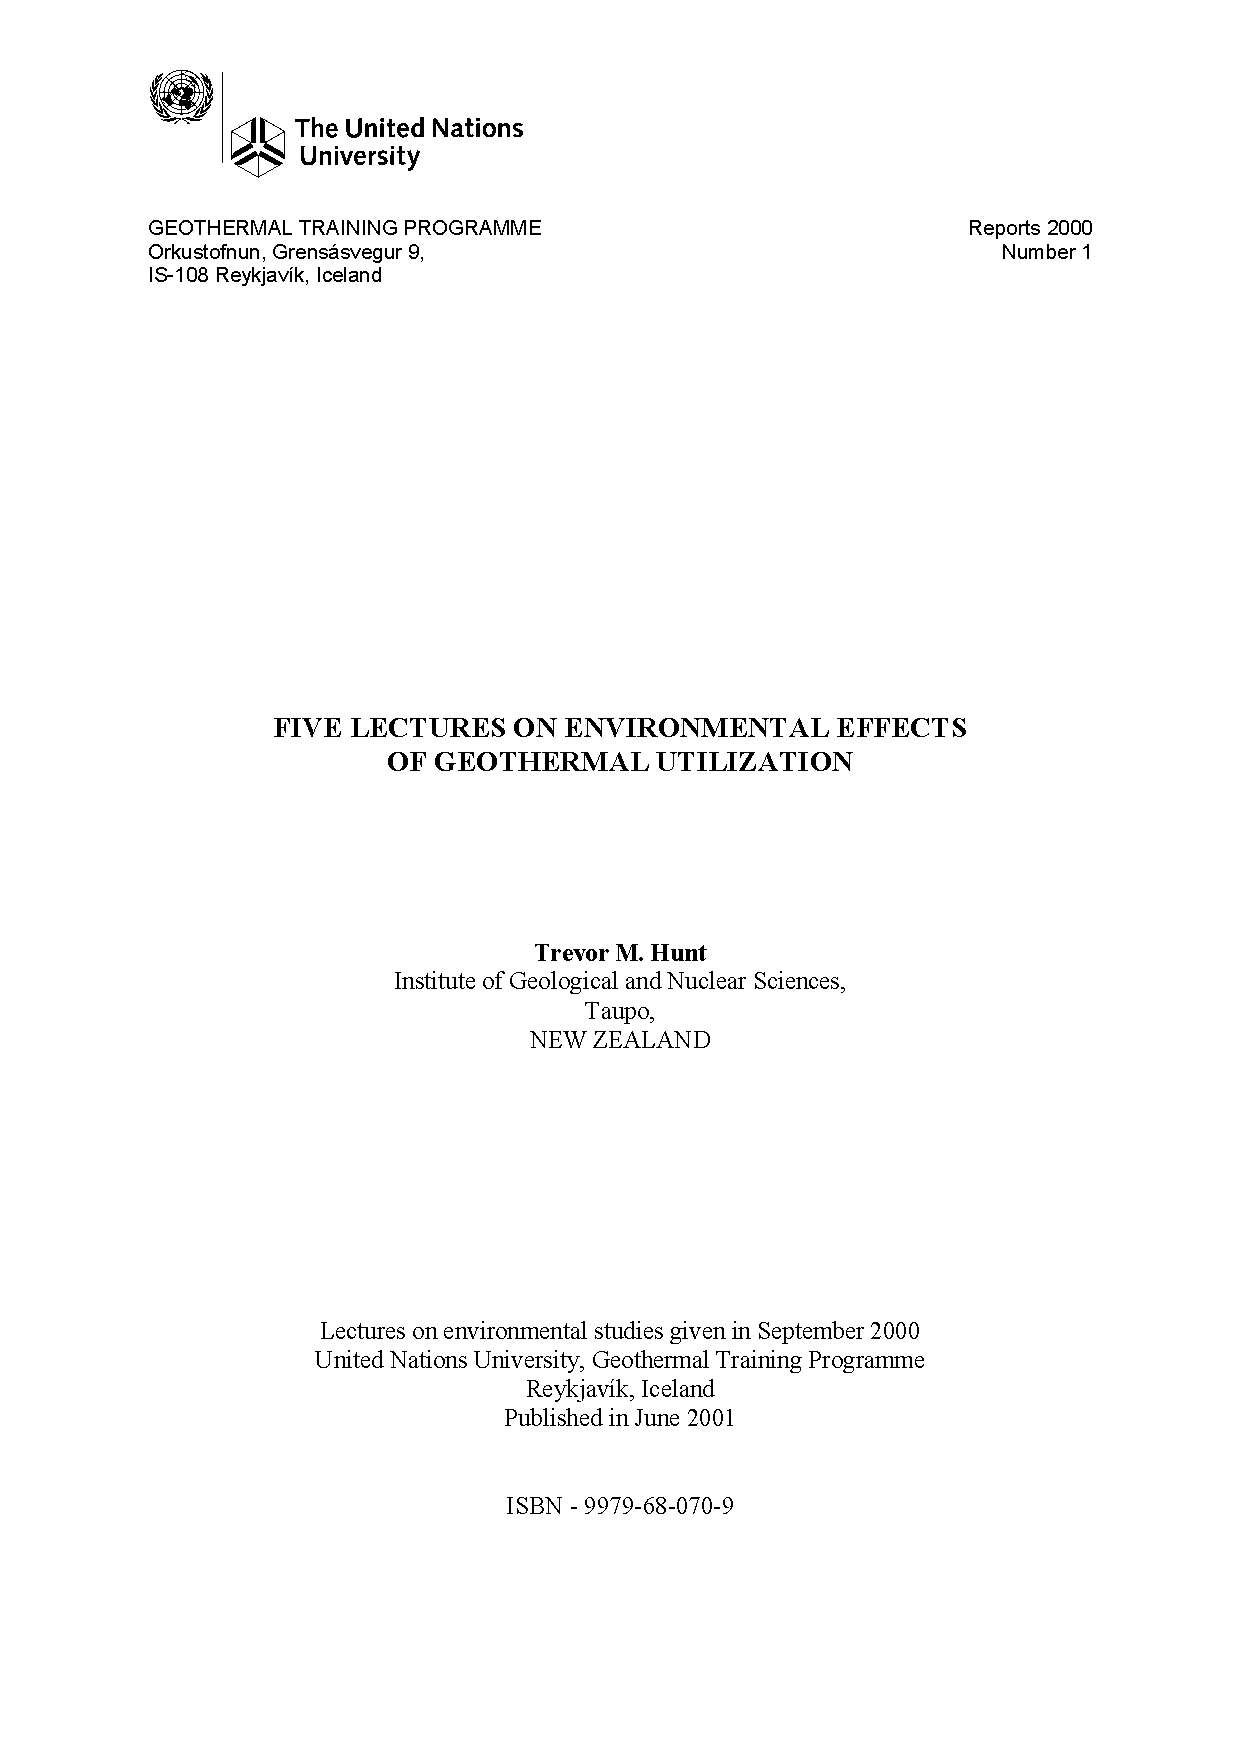
\includepdf[pages=-,fitpaper, angle=0]{./HuntSelect.pdf}
%}

\end{document}
